\documentclass[11pt,oneside]{amsart}
\usepackage{alttpreamble}
% \usepackage{tocloft}
% \renewcommand{\cftsecleader}{\cftdotfill{\cftdotsep}}
\begin{document}
\author{Maya Basu}
\author{Ethan Clayton}
\author{Fredrick Mooers}

\address{University of California, Berkeley}
\email{mab@berkeley.edu}

\address{University of Illinois, Urbana-Champaign}
\email{ewc3@illinois.edu}

\address{Virginia Tech}
\email{mooersfl24@vt.edu}

\title{Persistent Legendrian contact homology in $\R^3$}



\subjclass{53D42; 53D10, 57K10; 55N31}
\keywords{Legendrian contact homology, Legendrian knot, Persistent Homology}

\maketitle

\tableofcontents
\newpage

\section{June 17th: Flooding the Knot}

Consider a Legendrian Knot in the Lagrangian projection. The knot diagram is sectioned into \textit{patches}, enclosed (signed) areas, with total signed area zero. Given a patch in the knot diagram, pick a starting point on the boundary of the patch and travel counterclockwise around the boundary, marking each transverse double point (corner in the boundary) passed with a positive or negative sign depending on the Reeb sign. By Stokes' theorem, the signed sum of the Reeb heights of these double points must be strictly greater than zero.

\begin{definition}[Reeb Inequalities]
\label{def:ReebIneq}
The collection of inequalities (one for each patch) obtained in the manner above is called the \textit{Reeb inequalities}.
\end{definition}

\begin{example}[Trefoil Area]
\TODO: Add knot diagram.
    
\end{example}
\subsection{Algebraic Description}
Consider the set of all inequalities obtained by creating a chart for the knot. Follow the following procedure:
\begin{algorithm}
\label{alg:AlgFlood}
    \begin{enumerate} 
        \item Set $n = 1$
        \item Considering the (finite) collection of inequalities in the knot chart, find the generators $g_1 \cdots g_k$ which are only listed as positive terms in every inequality.
        \item Assign generators $g_1 \cdots g_k$ to tier $n$.
        \item Delete every inequality in the knot chart which contains at least one copy of any of the generators $g_1 \cdots g_k$.
        \item Increment $n$ by $1$, and repeat steps $2$ through $5$, until the knot chart is empty, meaning there are no remaining inequalities
        \item Any remaining generators not yet assigned to a tier are placed in the "extras" tier
    \end{enumerate}
\end{algorithm}

\subsection{Geometric Description}

Consider the set of all loops which are described by an inequality in the knot diagram. Label each corner of an intersection as $+$ or $-$ as whether traversing the intersection counterclockwise goes from an over-strand to an under-strand ($+$) or from an under-strand to an over-strand ($-$)

\begin{algorithm}
\label{alg:GeomFlood}
    \begin{enumerate} 
        \item Set $n = 1$
        \item Consider every generator $g_1 \cdots g_k$ where every negative corner of the crossing is in a shaded region. 
        \item Assign generators $g_1 \cdots g_k$ to tier $n$.
        \item Shade in ("flood") each region which is an area loop including these generators
        \item Increment $n$ by $1$, and start from step $2$, until the knot is completely flooded.
        \item The remaining generators are placed in the "extras" tier.
    \end{enumerate}
\end{algorithm}


Figure \ref{fig:Flood} shows the geometric flooding algorithm preformed on one of the Chekanov pairs, $m(5_2)$. The color brightness represent at what point in the algorithm the area loop was removed, with lighter coloring meaning being removed later.


\begin{figure}[htbp]
  \label{fig:Flood}
  \centering
  \includesvg{Pictures/CE2.svg}
  \caption{Flooding Algorithm on $m(5_2)$.}
\end{figure}


\subsection{Observations}





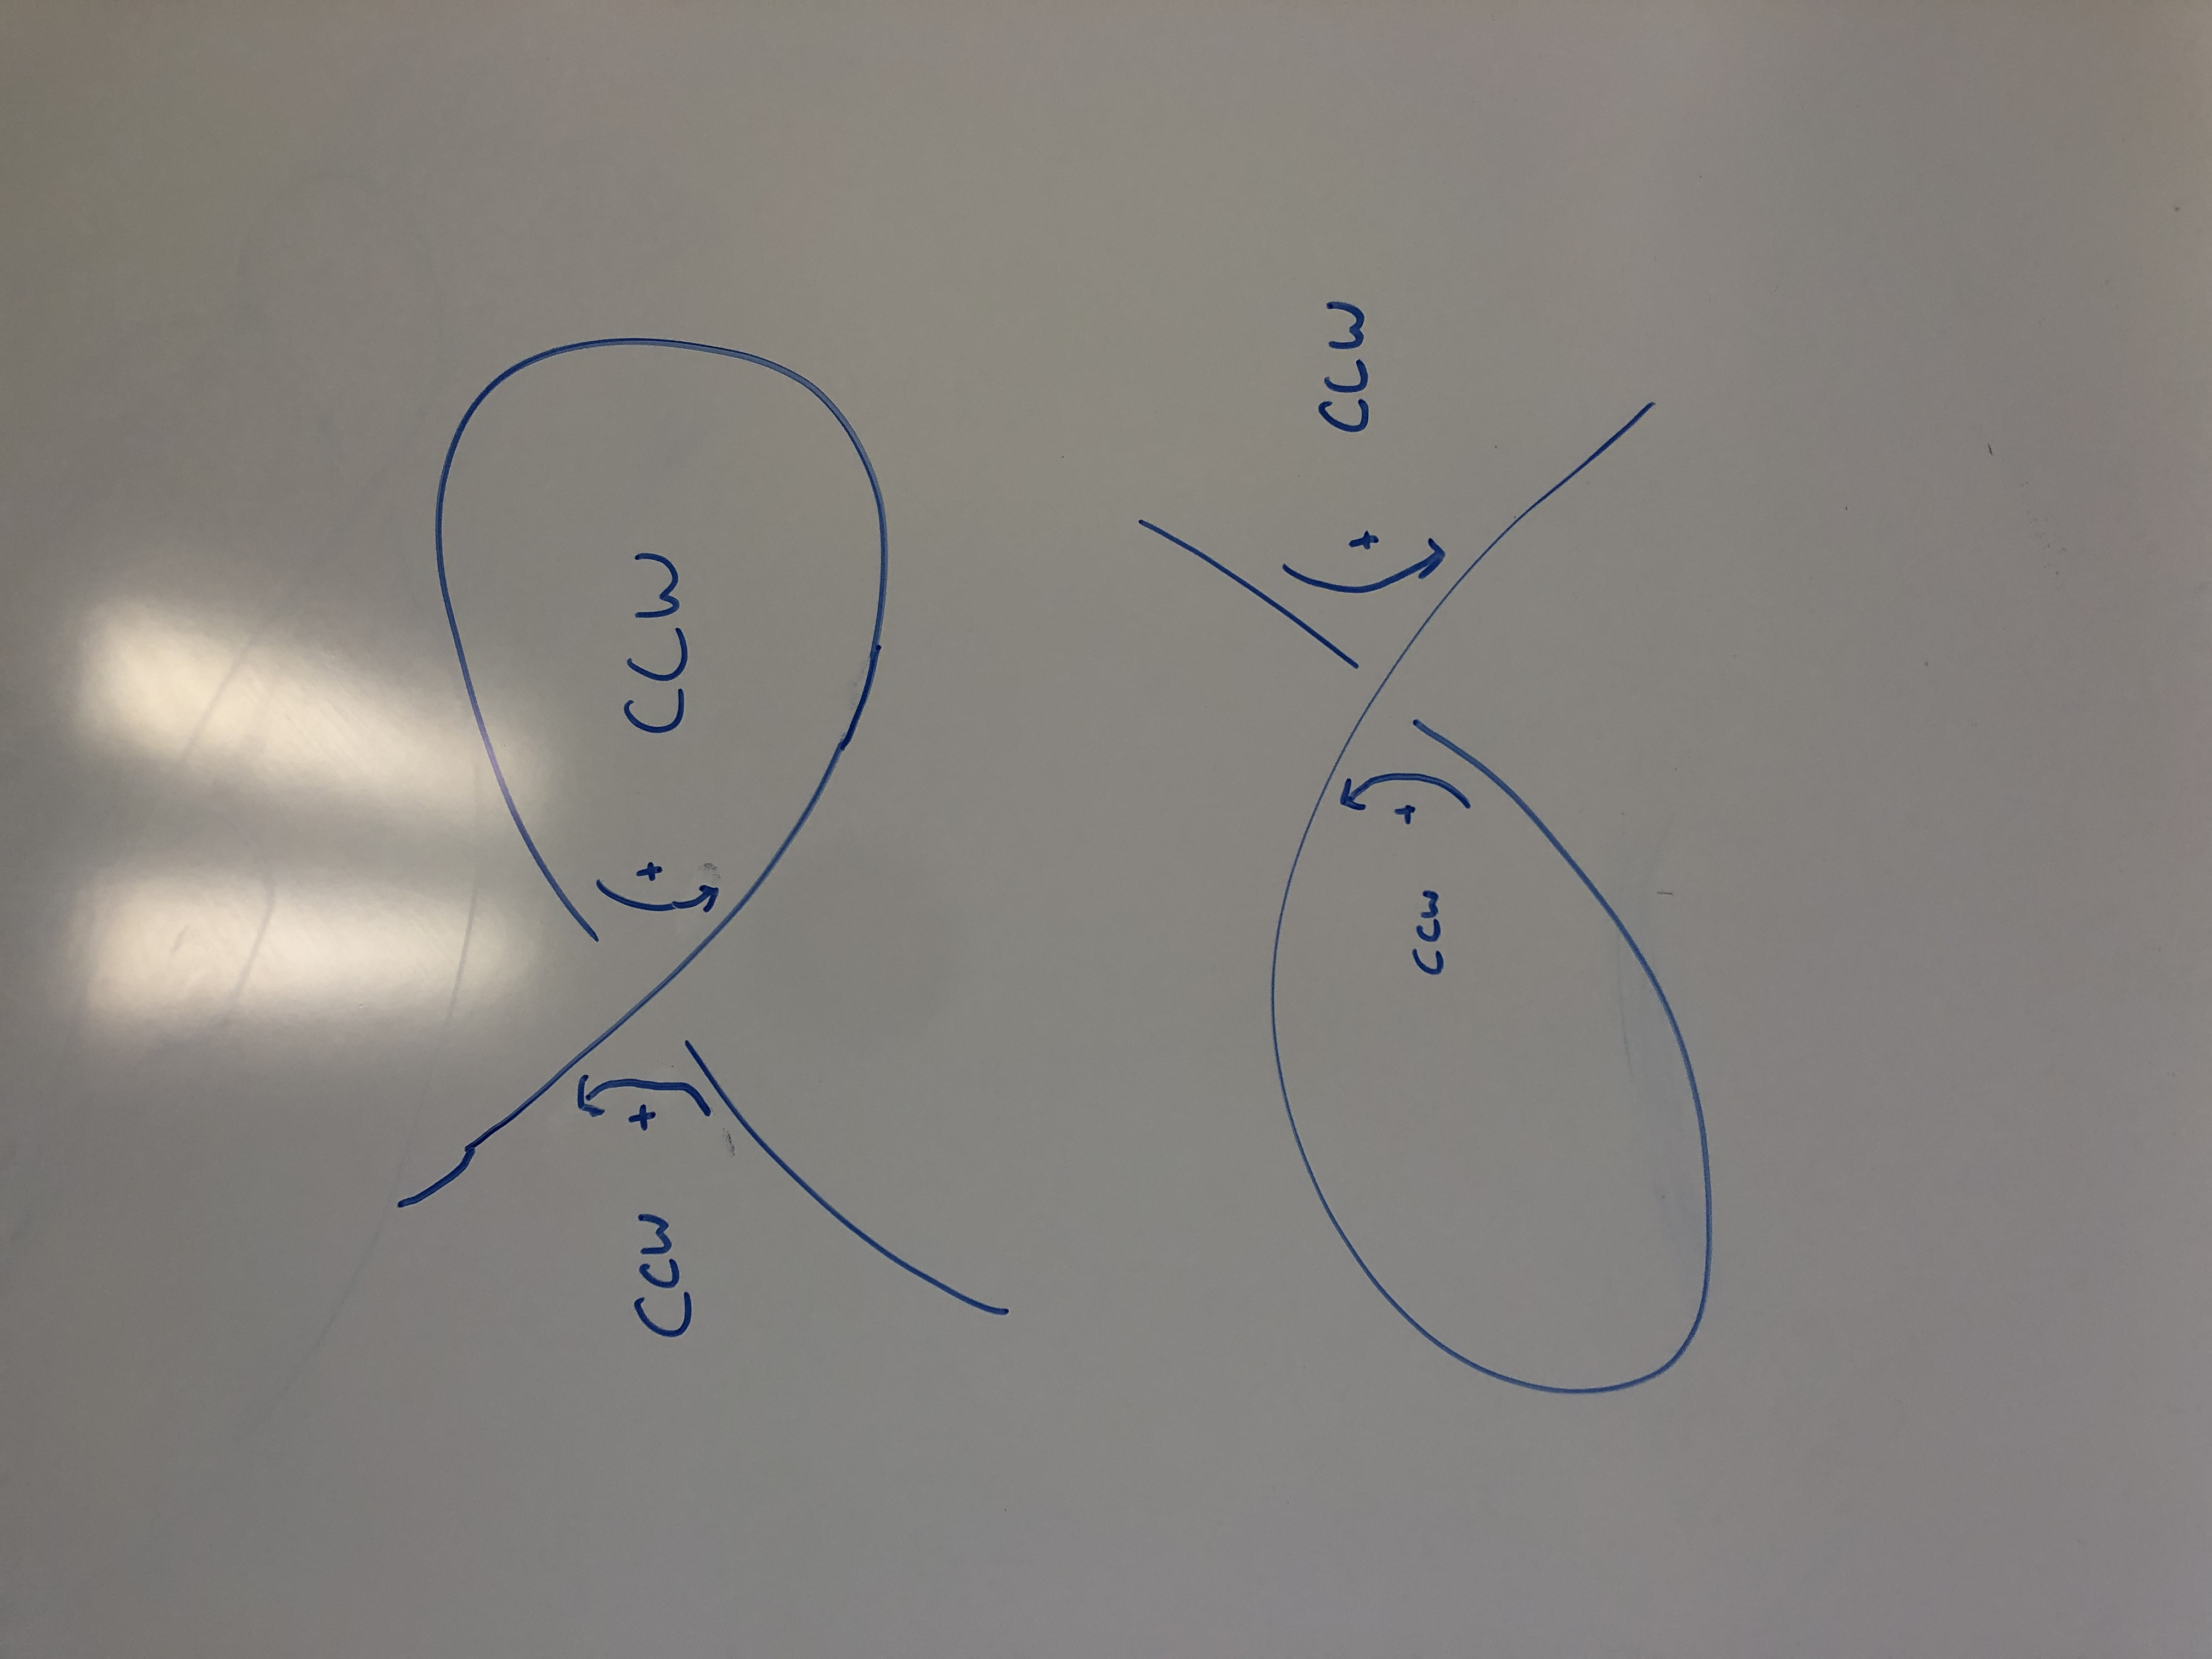
\includegraphics[width=4in,angle=-90]{Pictures/Exterior Loops.JPG}



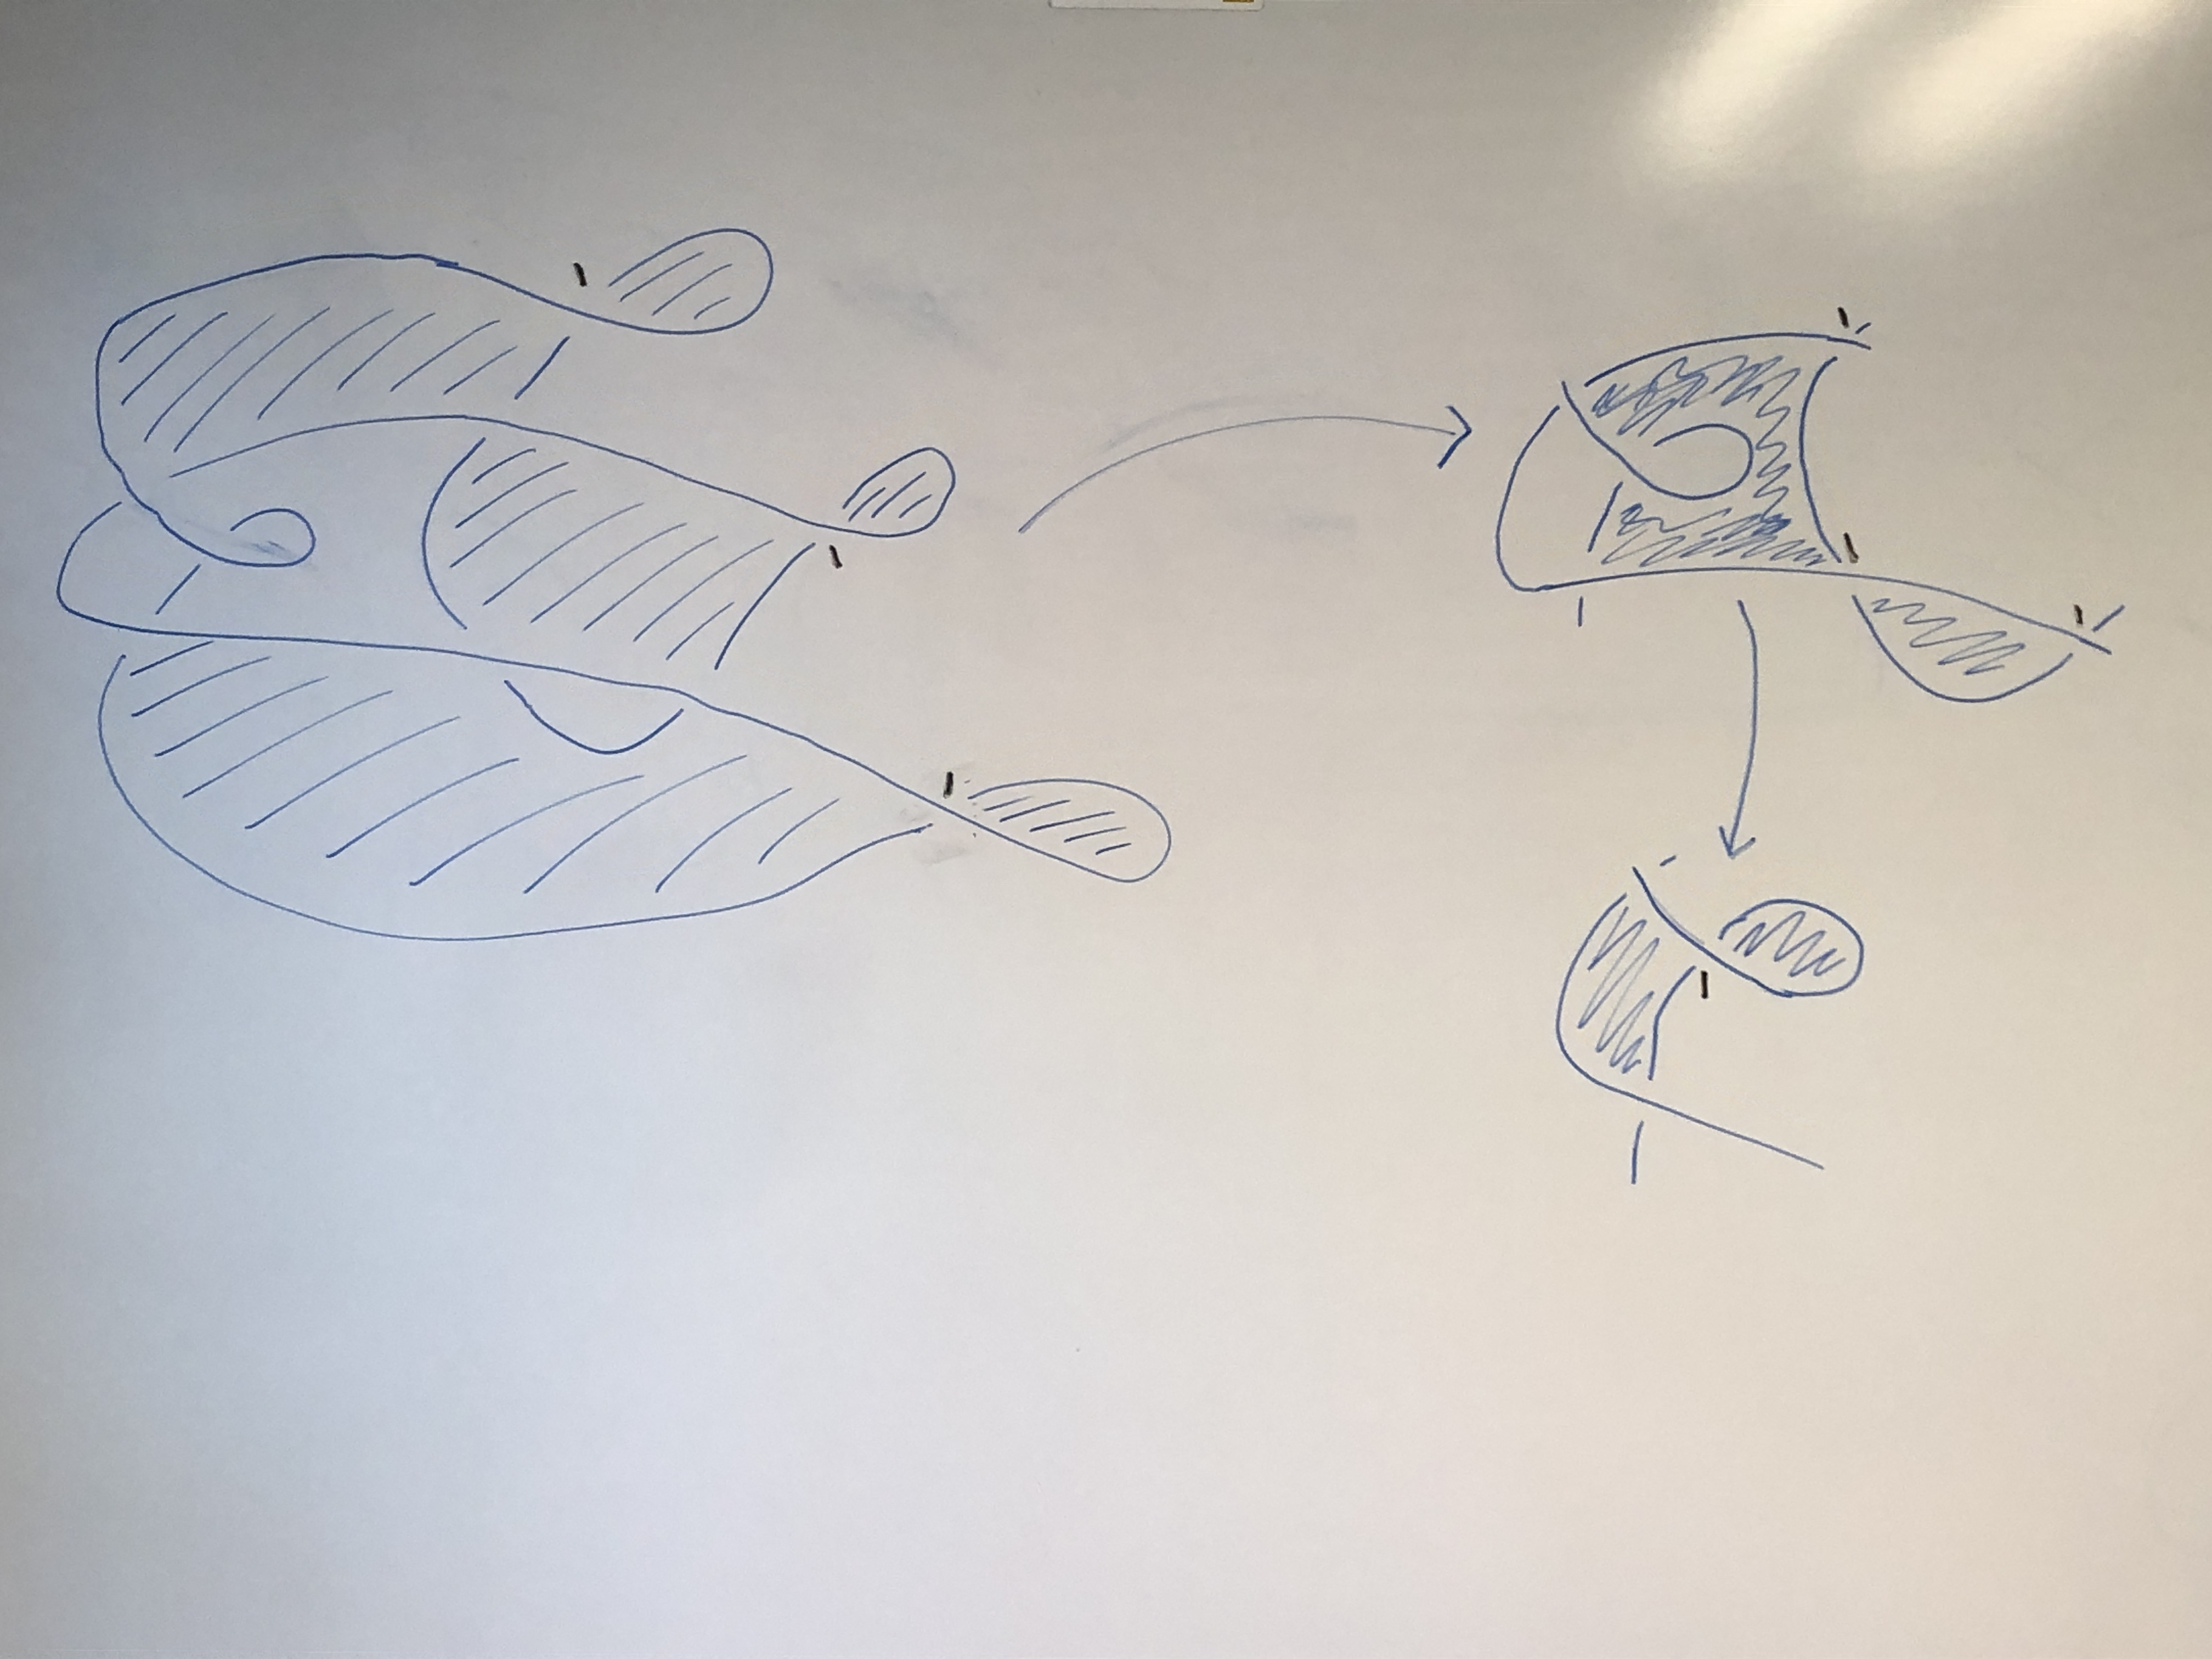
\includegraphics[width=4in]{Pictures/Visualization of Algorithm.JPG}

In this manner, continue through to the nth free generators, obtaining n classes of freedom, "the extras" are class n, which are never only positive in the remaining equations
\[f^{1}_1 \cdots f^{1}_{k_1} > f^{2}_1 \cdots f^{2}_{k_2}> \cdots > f^{n-1}_1 \cdots f^{n-1}_{k_{n-1}} > k_n \text{ extras }\]


\section{Assigning Heights}

Now we work backwards - assigning those in the extras class (these are all contractible, though not all contractible Reeb chords have to be nth free) to length 1, and then those in the $n-1$th class have length $k_n \cdot 1 + 1$ (+1 is so that we don't get exact equality) and those in the $n-2$nd class have length $ (k_n \cdot 1 + 1)\cdot k_{n-1} + 1$ and those in the $n-3$rd class $ ((k_n \cdot 1 + 1)\cdot k_{n-1} + 1)\cdot k_{n-2} + 1$ etc...




\subsection{Hypothesised equivalency for height lists of the same number of generators}

Perhaps an appropriate equivalency relation while include the following notion of equivalence:

Suppose that we have two classing systems of generators. Each produces many strict orderings of generators which still respect this class system. If the intersection of the set of strict orderings produced by two classing systems is nonzero, perhaps we should we consider these equivalent.




Further note:

These classes give us a filtration which is an action filtration with equities set at every opportunity. 







\section{June 19th: Proof of algorithm in a special case}


\begin{theorem}
    If a Legendrian Knot is in plat position and Ng's algorithm is applied, then for the resulting Lagrangian projection, our algorithm will always terminate.
\end{theorem}

\begin{proof}
    There are a finite number of total intersection within the knot. Therefore, if we can show that in each cycle of the algorithm, at least one intersection is placed into a tier, then the total number of remaining intersection is strictly decreasing and the algorithm must terminate.

    For any tier in the algorithm, consider the rightmost remaining intersection. It has two negative signs, above and below. By the nature of plat position, these negative signs are in a loop with a positive sign at an intersection to the right. Since by assumption those intersections are already cleared, the loops above and blow are filled in. Now there are two cases, either the intersection has only positive crossings remaining, or it is empty on the right and is thus an extra.

    If the intersection has only positive crossings remaining it is in the next tier and we are done. If the intersection is an extra then we must move to the next rightmost remaining intersection. Again this intersection has two negative signs, above and below which must have loops with positives to the right. The only intersections to the right are ones already covered or the extra we from the previous step. It a negative crossing has an extra to the right then it must be on an exterior loop since the extra is empty on the left. Otherwise, the negative crossing has an already covered positive to the right and is thus covered. In either case the new intersection has both negative crossings eliminated. Thus we are in the same position as before and the crossing is either in the next tier or an extra. If it is an extra we repeat this process until we find a non-extra or we have gone through all intersection.

    If we find an non-extra then it is placed in the next tier. Therefore each tier in the algorithm reduces the total number of remaining loops by one, and the algorithm must terminate. If there are no non-extras then all remaining intersections are places in the extras category and the algorithm also terminates. 
\end{proof}

\begin{figure}[htbp]
  \label{fig:PlatProof}
  \centering
  \includesvg{Pictures/proof1.svg}
  \caption{In plat, we trust.}
\end{figure}


Consider a knot in plat position which has two types of crossings. Considering a row (we call a region such as the one shaded below a "row", a strip where it ends in a loop).



there are crossings within rows and crossings between rows. Working our way from the right






Further observations:

All extras are "super" contractible (these are generators which are never responsible for shading a loop - therefore they can \textbf{all} be set equal to zero \textbf{simultaneously}.

Not all contractible chords are super contractible - some chords may go to zero iff one of the other positive generators in their loop increases by some finite amount. 


If there are no extras (super contractible chords) than the last class are contractible, as the lack of extras implies the last set of equations to be crossed out contains no negatives. 


Contractible chords can be in classes other than the last/extras class. For example, a stabilization introduced a contractible chord in the second class.

When attempting to 'swap' the heights of generators we observed that an element from a lower tier, can not be made greater than all of the heights of the tier above simultaneously, only some of them.

When doing Reidemeister move one in the front projection, we found that it added a single finite line to the bar-code in $H_0$, with a single (one element) generator. We hypothesize that this is always true, and so when finding an equivalence relation for bar-codes, we can 'mod out' theses types of lines. We will do more examples and test the other two Reidemeister moves.








\section{June 21st}


\subsection{Algebraic description of contractability}

\begin{definition}[Contractible]
    A Reeb chord $a$ is contractible if the Reeb inequalities still hold when the height of $a$ is set to $0$ (modulo disk inequalities \TODO)
\end{definition}

A contractible crossing is a generator $a_i$ in the area inequalities where for each inequality that $a_i$ appears as positive, there are no other negative terms, or if there is one or more negative terms, there is at least one other positive term.

This is a necessary condition for contractibility, but not sufficient, as if we take the "actual" definition of contractibility to be a legandrian isotopy up to the endpoint where the height goes to zero. This can not happen if the above requirement is not satisfied, however, the above requirement does not automatically guarantee the existence of such a legendrian isotopy. 

\begin{lemma}
    \label{lem:extradesc}
    For a Legendrian $\L$ with $F(\L)$ in plat position, the extras of the flooding algorithm are crossings that eventually look like ``pinch crossings''
\end{lemma}
\begin{proof}
    Algebraic v. Geometric picture clear \TODO
\end{proof}

\begin{definition}
    \label{def:doubleshade}
    A crossing $a$ in $F(\L)$, that isn't an extra of the flooding algorithm, \textit{double shades at tier $n$} if every inequality at the $n$th step of the flooding diagram that $a$ appears in contains another Reeb height with positive sign. If $a$ double shades at all tiers, we say $a$ double shades.
\end{definition}

% \begin{lemma}
%     For $F(\L)$ in plat position, a crossing double shades or is an extra at tier $n$ for some $n$ if and only if it double shades or is an extra at all tiers.
% \end{lemma}

\begin{lemma}
    \label{lem:doubleshadecrit}
        For $F(\L)$ in plat position, a crossing double shades at tier $1$ if and only if it double shades at all tiers.
\end{lemma}
\begin{proof}
    The forward direction is trivial. For the backwards direction, not that if $a$ double shades at tier $1$, then it double shades at least until it's removed at tier $n$. If there is a patch to the left of $a$, then we're done. If there isn't a patch to the left of $a$ then note that the crossing on the other side of the patch to the right of $a$ (when a left crossing exists a right cusp or crossing to the right exists) also exists while $a$ is breathing. If this weren't the case, then $a$ would be negative in all Reeb inequalities at time $n$ and thus making it an extra. Hence, $a$ drowns with its right patch flooding meaning $a$ double shades for all tiers.
\end{proof}

\begin{proposition}
    \label{prop:contractdesc}
    For $F(\L)$ in plat position, a Reeb chord corresponding to a right cusp or double point, $a$, is contractible if and only if $a$ double shades or is an extra or corresponds to a left loop in $\Pi(\L)$.
\end{proposition}

\begin{proof}
    ($\Rightarrow$) Assuming that $a$ doesn't double shade, we must show that $a$ is never removed by the flooding algorithm (i.e. $a$ is an extra) or is removed at the last step on the algorithm (i.e. $a$ corresponds to a left loop in $\Pi(\L)$). Since $a$ is contractible, the patch to the left, if it exists, corresponds to an inequality that has no negatives. Such an inequality can exist precisely when $a$ corresponds to a left loop in $\Pi(\L)$. If a left patch doesn't exist, then since $a$ doesn't double shade, it follows that a right patch at a certain step in the algorithm floods before the algorithm terminates, and hence $a$ is an extra.

    ($\Leftarrow$) Clearish?
\end{proof}

\begin{corollary}
    \label{cor:contractenum}
    The flooding algorithm enumerates contractible Reeb chords for a legendrian $\L$ with $F(\L)$ in plat position.
\end{corollary}


\subsection{Stabilization}
Adding a stabilization with generator $a_j$ creates a contractible reed chord, because we add two things to the area inequalities: $a_j>0$ and we add a positive $a_j$ to one other area inequality. Because we previously had a valid knot, there must have been at least one other positive in this latter equation, so the added $a_j$ satisfies the necessary conditions of contractibility. 

\section{June 26th}

\subsubsection{Reidemeister move F1}

The first Reidemeister move in the Front Projection, now called F1, connects two Legendrian Isotopic Knots. It adds two generators, called $a_i$ and $a_j$, with gradings 1 and 0 respectively. $\d (a_i) = 1 + a_j$ and $\d (a_j) = 0$. Furthermore, this operation does not destroy or create and disks which define the differential for the other generator, though it may add $a_j$ to some disks. As a result, it leads to a small change in the bar-code generated by the persistence homology. Namely, it adds a single, finite, singularly generated line to the bar-code picture in $H_0$. It may also lead to the relabeling of some generators on other lines (almost certainly only those in $H_1$.


\subsubsection{Reidemeister move F2}

Hypothesis: The second Reidemeister move in the Front Projection, on Left Cusps, adds two generators $a$ and $b$ with $\d a = b$ and $\d b = 0$. The new generators may be added into other differentials, however, after the height tier which adds $a$, the (truncated) barcode will will look like the same as the original barcode killed off by $\text{\d(original generators} + a)$ whenever $b$ appears is a factor in the original generators differential.\footnote{This is if the augmentations are 'preserved' in the way we would like.} 

See picture for proofs of why differentials don't change all that much. The stuff on the exterior to the left is unaffected, and the stuff to the right is also unaffected. It's *probably* not possible to have a disk in the interior since to move CCW you must inevitably hit a right cusp which would have a positive sign. So, all in all, nothing can be removed from original differentials, only can be added, corresponding to the tame isomorphism. The previous 2 sentences give a reason for why $\d a=b$, since any other disk needs to hit a right cusp in order to move CCW. All in all, moving right-to-left is harder than left-to-right.



\subsubsection{Reidemeister Move F3}

The third Reidemeister move, given the natural renaming of generators (where the middle crossing stays the same and the two side crossing switch places, following the middle strand sliding through) induces a map between the DGAs of the two knots. With the following nomenclature we have: (For Mod 2 only!)

\[a_1 \rightarrow a_1\]
\[a_2 \rightarrow a_2\]
\[a_3 \rightarrow a_3 + a_2a_1\]
The proof of this is gotten by considering how each generator can possible be included in a differential disk, and seeing that under this transformation, these disks are transformed appropriately. Because of mod 2, this map works both ways between the two positions of the move.


\begin{lemma}

A tame isomorphism induces a map between non-linear DGAs. What is the corresponding map between linearized DGAs that would complete the commutative diagram?

Assume that we wish to consider the tame isomorphism $a_k \rightarrow a_k + u$ (all other generators left unchanged), and assume that $u \neq 1$, and $\epsilon(a_k) = 0$. Additionally, take the map of augmentations to be $\epsilon(g) = \epsilon'(g)$ for $g \neq a_k$, and $\epsilon(a_k) = \epsilon'(a_k + u)$. Consider the non linear DGA consisting of differentials 
\[\partial x_i = \sum_{j} (g_{1j} \cdots a_k \cdots g_{nj}) + \mathcal{O}\]
where the first sum 


    
\end{lemma}





\section{June 28th}

\subsection{Stablization}

    Any Legendrian Isotopy of knots induces a stable time Isomorphism at the level of DGA's.  We planned to examine the effects that stabilizations and tame isomorphisms have on the persistence module barcode, to understand which parts are homologically significant. 
    
    We found that a grading K stabilization, adds a single finite bar to $H_(k-1)$ which is generated by a single element. On the level of DGA's, a grading K stablizations adds two generators $e_k$ and $e_(k-1)$. $e_k$ has grading $k$ and $e_(k-1)$ has grading $k-1$, and their differentials are given by $\d (e_k) = 1 + e_(k-1)$ and $\d e_(k-1) = 0$. After linearizing this must give linear differentials $\d^\epsilon (e_k) = e_(k-1)$ and $\d^\epsilon e_(k-1) = 0$. 

    $e_(k-1)$ causes a finite bar to be born at time $h(e_(k-1))$. and since $\d^\epsilon (e_k) = e_(k-1)$, this bar dies at time $h(e_k)$. This bar has generator $e_(k-1)$. This Stabilization also has no effect on any other differentials, so it does not alter any other bars, finite or otherwise.

\subsection{Tame Isomorphisms}

    A tame isomorphism can change the number of generators for any bar. For example, if a bar is generated by $a_1 + \cdots a_n$, then we can have a tame isomorphism that sends $a_1$ to $a_1 + a_2 + \cdots a_n$, and all other generators to themselves. After this tame isomorphism, the bar will be generated by $a_1$.

\subsection{New Hypothesis}

Wild Speculation:
    After doing an example we believe we have a new way to define homologically inessential and essential.

    \begin{definition}
        For a persistence module barcode we call a finite bar $H$-contractible, if there is a valid assignment of heights to Reeb chords such that for any $\epsilon > 0$
        \begin{enumerate}
            \item For any Reeb Chord $a_i$, the height $h(a_i) \geq 1$
            \item the length of the bar $l < \epsilon$
        \end{enumerate}
    \end{definition}

    We claim that any $H$-contractible bar is homologically inessential, and that any bar which is not $H$-contractible is homologically essential.

$H$-contractible bars are by definition invariant under planar isotopy, since planar isotopy only corresponds to a reassignment of Reeb heights.

Observation: When doing a Reidemeister move 2 onto the trefoil, we added a new $H$-contractible bar. We also altered the existing finite bar. However it remained not $H$-contractible, which is a good sign. That bar is born at the max of $a_3$ and $a_5$, and is killed either by $a_2$ of $a_1$ and $b_2$. However, we have that $a_2$ must be larger than $a_3 + a_4 + a_5$ and $a_1$ must be larger than $b_1 + a_3 $ and $b_2$ must be larger than $a_4 + a_5$. (+ > max).

Problem: We found that if you do a Front projection Reidemeister move 1, and then a second Front projection Reidemeister move 1 on top of the previous move, the previous $H$-contractible bar that was created by the first move is made not $H$-contractible by the second move. This is because the differential is altered. This gives us a new definition

    \begin{definition}
        For a persistence module barcode we call a finite bar $H$-contractible, if there is a valid assignment of heights to Reeb chords such that for any $\epsilon > 0$
        \begin{enumerate}
            \item For any Reeb Chord $a_i$, if $a_i$ is not contractible, the height $h(a_i) \geq 1$
            \item the length of the bar $l < \epsilon$
        \end{enumerate}
    \end{definition}

\section{Questions?}

\subfile{General-Information/questions?.tex}

\section{Examples}

\subfile{General-Information/examples.tex}

\section{Observations}





what to do with finite length bars which have a mix of generators

relation between extras and 1st Reidmeister moves

can any front projection knot be turned into grid position with only planar isotopy, no reidemister moves (if so, this could be used to prove that height algorithm terminates for any knot)






\end{document}